\documentclass[]{book}

% QCC book needs
\usepackage{fix-cm}  % this package allows large \fontsize
\usepackage{imakeidx}
\makeindex[title=Index]
\usepackage{listings}
\usepackage[table]{xcolor}

\usepackage{amsmath,graphicx}

\usepackage{tikz}    % this is for graphics. e.g. rectangle on title 
\usetikzlibrary{quantikz, decorations.pathmorphing,shapes.geometric}
%\usepackage{circuitikz}
\usepackage{tikz-3dplot} % includes tikz
\tdplotsetmaincoords{70}{120}
\usepackage{float}


% This file is for commands / macros / functions.
% QCC book specific
\newcommand{\keta}[2][]{\vert {#2} \rangle_{#1}}
\newcommand{\braketa}[3][]{\langle {#2} \vert {#3}\rangle_{#1}}

\tikzstyle{Gate}=[rectangle, minimum width=30, minimum height=30, text width=20, text centered, draw=black]
\usepackage{pgfplots}
\usepgfplotslibrary{fillbetween}

\begin{document}


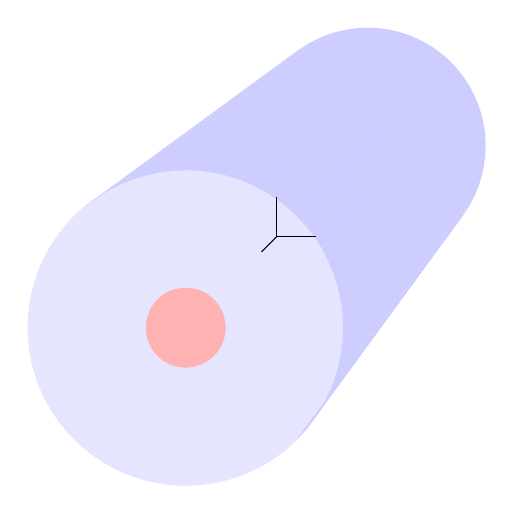
\begin{tikzpicture}[scale=0.5]
    \def\R{4} % Outer radius
    \def\Rb{3} % Outer radius
    \def\r{1} % Inner radius
    \def\L{6} % Half Length of the tube
    \def\S{4.2} % half Shift distance between tubes
    \def\I{5} % increment

    % Left tube
    \draw[blue!10,fill] (0,0,\L) circle (\R);   
    \draw[red!30,fill] (0,0,\L) circle (\r);    
    %\draw[decorate,decoration=zigzag] (-\S,0,-\L) circle (\Rb);
%    \foreach \t in {-40,-35,...,123} {
%        \fill[blue!20] ({\R*cos(\t+\I)}, {\R*sin(\t+\I)}, \L) -- ({\R*cos(\t)}, {\R*sin(\t)}, \L) 
%        -- ({\Rb*cos(\t)}, {\Rb*sin(\t)}, -\L) -- ({\Rb*cos(\t+\I)}, {\Rb*sin(\t+\I)}, -\L) -- cycle;
    \foreach \t in {-45,-40,...,125} {
        \fill[blue!20] (xyz cylindrical cs:radius=\R, angle=\t, z=\L) -- (xyz cylindrical cs:radius=\R, angle=\t+\I, z=\L) -- (xyz cylindrical cs:radius=\Rb, angle=\t+\I, z=-\L) -- (xyz cylindrical cs:radius=\Rb, angle=\t, z=-\L)        -- cycle;
    }

  \draw (0,0,0) -- (xyz cylindrical cs:radius=1);
  \draw (0,0,0) -- (xyz cylindrical cs:radius=1,angle=90);
  \draw (0,0,0) -- (xyz cylindrical cs:z=1);

%    \begin{axis}
%      \addplot3+[data cs=polarrad,domain=0:2*pi] (\x,1,2*\x);
%    \end{axis}
    
\end{tikzpicture}

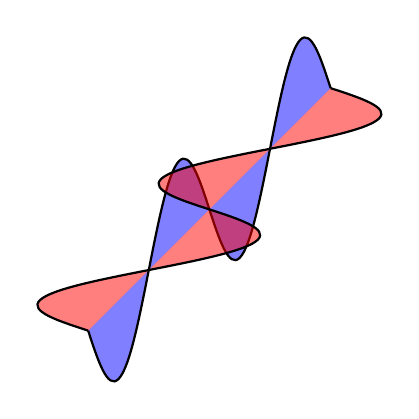
\begin{tikzpicture}%[z={(10:10mm)},x={(-45:5mm)}]
  \def\wave{
    \draw[fill,thick,fill opacity=0.5]
     (0,0) sin (1,1) cos (2,0) sin (3,-1) cos (4,0)
           sin (5,1) cos (6,0) sin (7,-1) cos (8,0);
           %sin (9,1) cos (10,0)sin (11,-1)cos (12,0);
%    \foreach \shift in {0,4,8}
%    {
%      \begin{scope}[xshift=\shift cm,thin]
%        \draw (.5,0)  -- (0.5,0 |- 45:1cm);
%        \draw (1,0)   -- (1,1);
%        \draw (1.5,0) -- (1.5,0 |- 45:1cm);
%        \draw (2.5,0) -- (2.5,0 |- -45:1cm);
%        \draw (3,0)   -- (3,-1);
%        \draw (3.5,0) -- (3.5,0 |- -45:1cm);
%      \end{scope}
%    }
  }
  \begin{scope}[canvas is zy plane at x=0,fill=blue]
    \wave
%    \node at (6,-1.5) [transform shape] {magnetic field};
  \end{scope}
  \begin{scope}[canvas is zx plane at y=0,fill=red]
%    \draw[help lines] (0,-2) grid (12,2);
    \wave
%    \node at (6,1.5) [rotate=180,xscale=-1,transform shape] {electric field};
  \end{scope}
\end{tikzpicture}

\end{document}